\documentclass[a4paper,11pt]{article}
\usepackage[a4,bmtuk,themeblue]{tuepdfscreen2008}
\usepackage[english]{babel}
%\usepackage{amsmath}      % not required in every poster, only those which use amsmath commands (like \DeclareMathOperator)
%\usepackage{mathtime}     % This package is not required, it loads Mathtime fonts for mathematical formulas which I prefer.
\setstatustext{
\includegraphics[height=1.2cm]{IMAGe.png}}       % This text is placed in the upper left corner of the poster and can be left empty
\titlelogo[height=4cm]{veronika_details.png}               % You can use this command to insert one logo.

%\titleright{v.cheplygina@tue.nl  http://www.veronikach.com}
%\titleright{
\includegraphics[height=1.2cm]{veronika_details.png}}


\definecolor{myblue}{rgb}{.0,.0,.8}
\newcommand{\myblue}[1]{\textcolor{myblue}{#1}}

\definecolor{myred}{rgb}{.8,.0,.0}
\newcommand{\myred}[1]{\textcolor{myred}{#1}}

\begin{document}
\begin{slidetop}
\slidetitle[Veronika Cheplygina, Pim Moeskops, Mitko Veta,\\ Behdad Dashtbozorg, Josien P.W. Pluim]{Exploring the similarity of medical imaging classification problems}
\begin{multicols}{2}

\section*{Introduction}

\begin{itemize}

\item You have experience with medical imaging problems A and B. Your colleague asks for advice about what classifier to use for problem C

\item Your advice is based on similarity of C to A and B. How can we quantify this similarity?

\item Let's represent problems A, B and C in the same feature space (meta-learning)

\end{itemize}




\section*{Method}

\begin{itemize}

\item Assume we are given $\{(D_i, M_i)\}_{1}^{n}$, where $D_i$ is a dataset from A, B or C and $M_i$ is a meta-label, such as the best complex classifier.

\item Represent each dataset $D_i$ by (normalized) performances of $k$ simple classifiers

\item Embed the $n\times k$ representation in 2D. If clusters reflect labels $M_i$, could potentially predict best complex classifier for unseen problems

    \end{itemize}


\begin{center}
  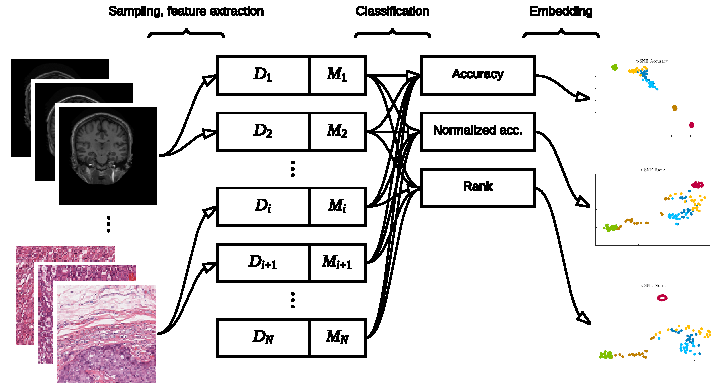
\includegraphics[width=0.9\columnwidth]{overview.pdf}%
  \figcaption{Overview of the method}
  \label{fig:mil}
\end{center}



\section*{Experiments}

\footnotesize

\begin{center}
\begin{tabular}{l l l l l}
\hline
Dataset & Type & Images & Features \\
\hline

Tissue & Brain MR & 20 &  768, CNN \\
Mitosis & Histopathology & 12 &  200, CNN \\
MitosisNorm & Histopathology & 12 &  200, CNN \\
Vessel & Retinal & 20 & 29, Classical \\
ArteryVein & Retinal & 20 &  30, Classical \\
Microaneurysm & Retinal & 381 & 30, Classical\\
\hline
\end{tabular}
\label{tab:datasets}
\figcaption{Six segmentation problems used in the experiments.}
\end{center}

\normalsize

\begin{itemize}
\item Sample 20 $\times$ from 6 segmentation problems, for a total of $n=120$ datasets. Define $M_i$ as the segmentation problem, i.e. Tissue etc. (Ask me about the assumptions!)

\item Classifiers ($k=6$): nearest mean, \{linear, quadratic\} discriminant, logistic regression, 1-nearest neighbor and decision tree. 

\item Normalize accuracies for each of the $n$ rows between 0 and 1, or by ranking between 1 and 6

\item t-Stochastic Neighbor Embedding (t-SNE) and multidimensional scaling (MDS) for embedding


\end{itemize}



\begin{center}
	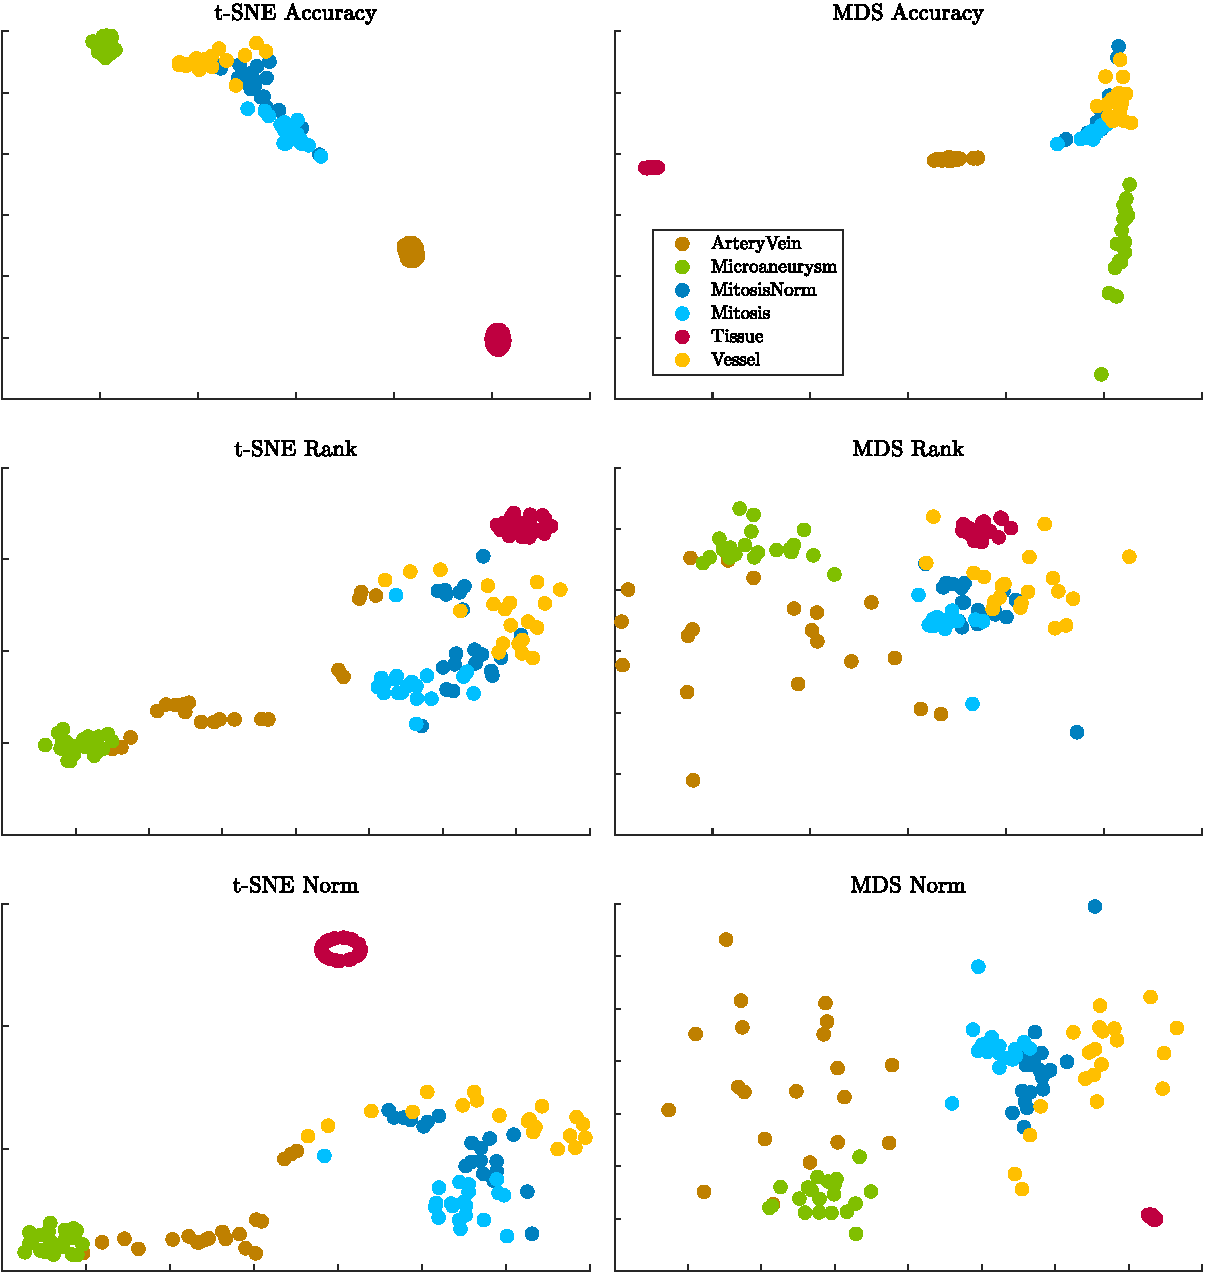
\includegraphics[width=0.8\columnwidth]{embedding.pdf}
	 \figcaption{2D embeddings with t-SNE and MDS for datasets from 6 classification problems}
  \label{fig:example}
\end{center}



\section*{Discussion}

\begin{itemize}

\item Clusters reflect the artificial labels $M_i$, representation is promising for quantifying similarity of datasets

\item Further experiments needed with real $M_i$ labels

\item Feature extraction should be included in $M_i$, not predefined

\end{itemize}

\footnotesize
%Cheplygina, V., S{\o}rensen, L., Tax, D. M., de Bruijne, M., \& Loog, M. (2015). Label stability in multiple instance learning. In International Conference on Medical Image Computing and Computer-Assisted Intervention (MICCAI) (pp. 539-546).


%\item \texttt{v.cheplygina@tue.nl  \url{http://www.veronikach.com}}

%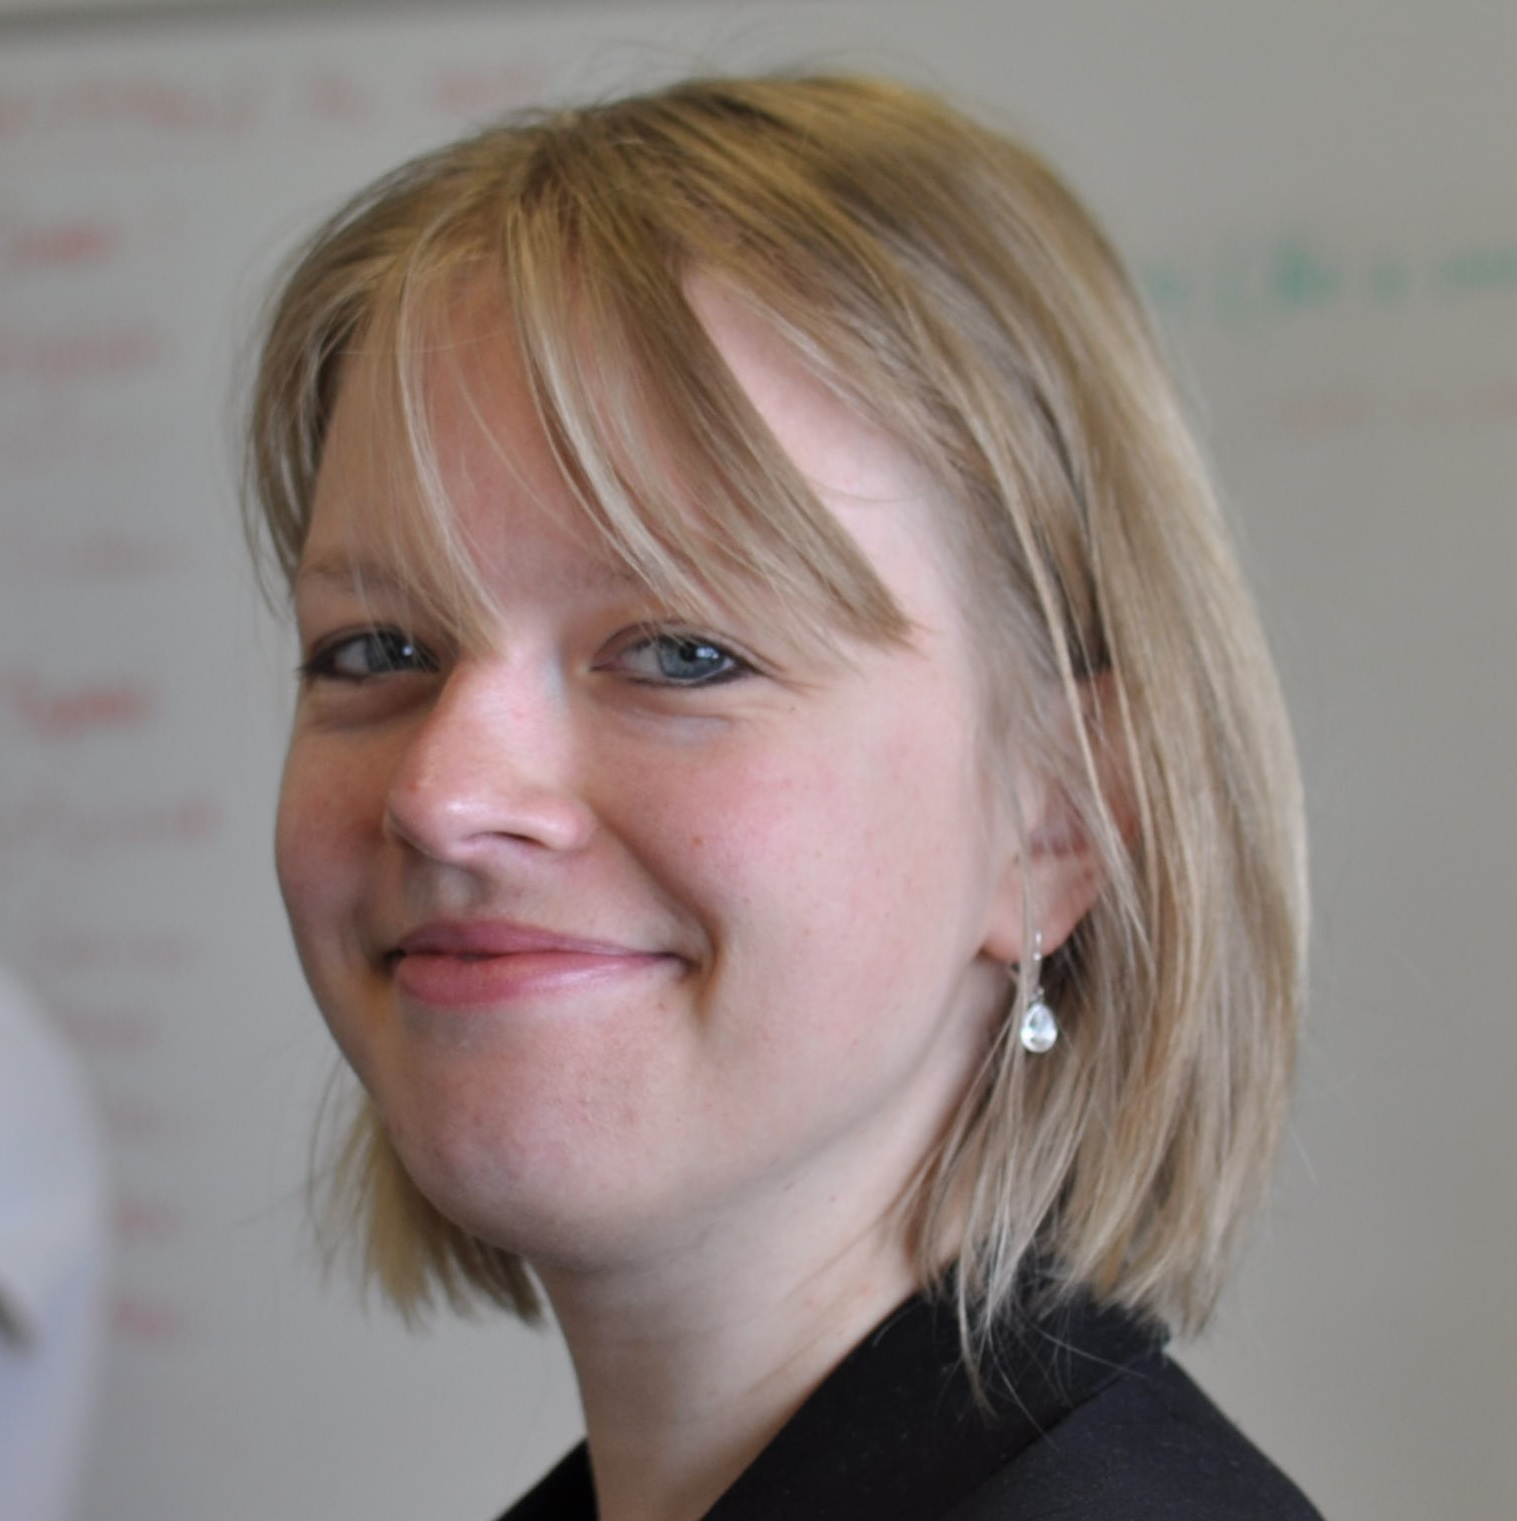
\includegraphics[width=0.2\columnwidth]{../figures/veronika.jpg}
%
\includegraphics[width=0.4\columnwidth]{IMAGe.png}





\end{multicols}
\end{slidetop}

\end{document}

